\subsection{Задание 4. Зависимость отношения сигнал/шум на выходе согласованного
фильтра от параметров входного сигнала}

В задании исследуется свойство системы с согласованным фильтром при различных
параметрах ЛЧМ сигнала: девиации частоты $\Delta f_{\text{дев}}$ и длительности
сигнала $\tau$.

\subsubsection{Однократный замер}%
\label{ssub:odnokratnyi_zamer}



\paragraph{Изменяющаяся длительность ЛЧМ сигнала}%
\label{par:izmeniaiushchaiasia_dlitel_nost_signala_tau_}

Установили девиацию частоты $\Delta f_{\text{дев}}= 700$ Гц и изменяли частоту
в пределах 10 мс -- 100 мс. 

Для одной реализации виртуальным прибором
вычислялось отношение сигнал/шум. Получившаяся зависимость приведена на рис.
\ref{fig:4.1}

\begin{figure}[h!]
    \centering
    %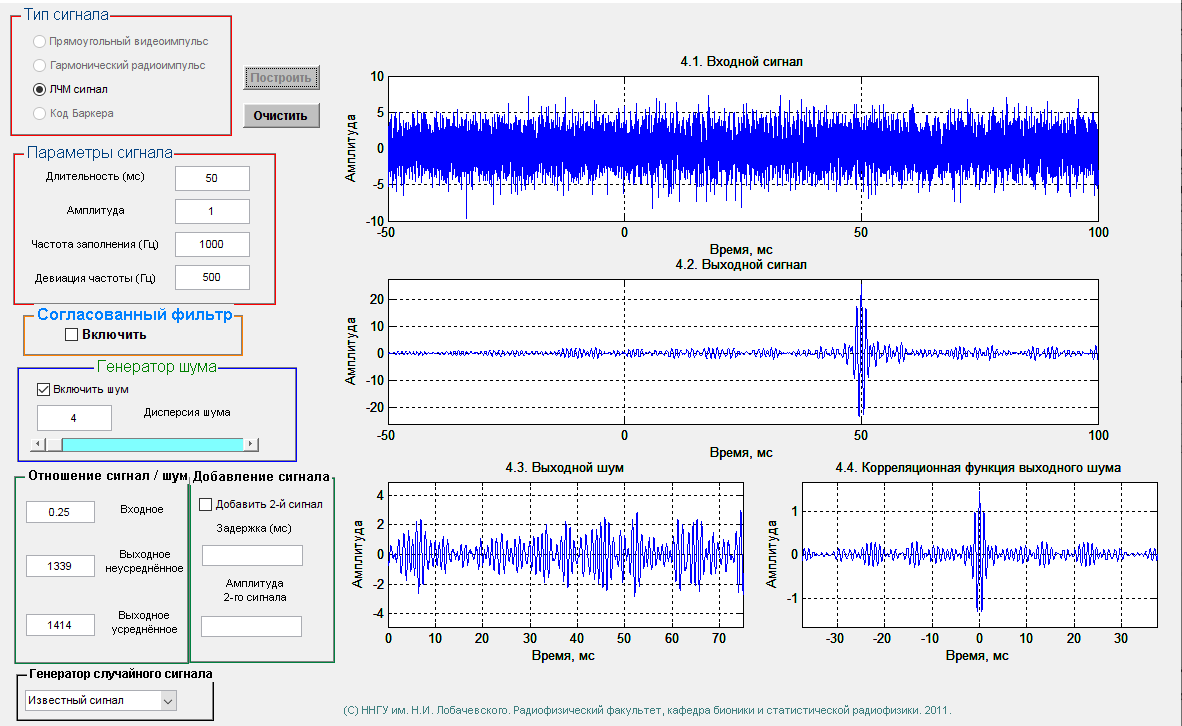
\includegraphics[width=0.6\linewidth]{imgs/t4s4_500}
    \includegraphics[width=0.6\linewidth]{example-image-a}
    \caption{}
    \label{fig:4.1}
\end{figure}

\paragraph{Изменяющаяся девиация частоты ЛЧМ сигнала}%
\label{par:izmeniaiushchaiasia_deviatsiia_chastoty_signala}
Установили длительность сигнала $\tau=50$ мс и изменяли девиацию в пределах
400 Гц - 1000 Гц.

Для одной реализации сигнала виртуальным прибором
вычислялось отношение сигнал/шум. Получившаяся зависимость приведена на рис.
\ref{fig:4.2}

\begin{figure}[h!]
    \centering
    %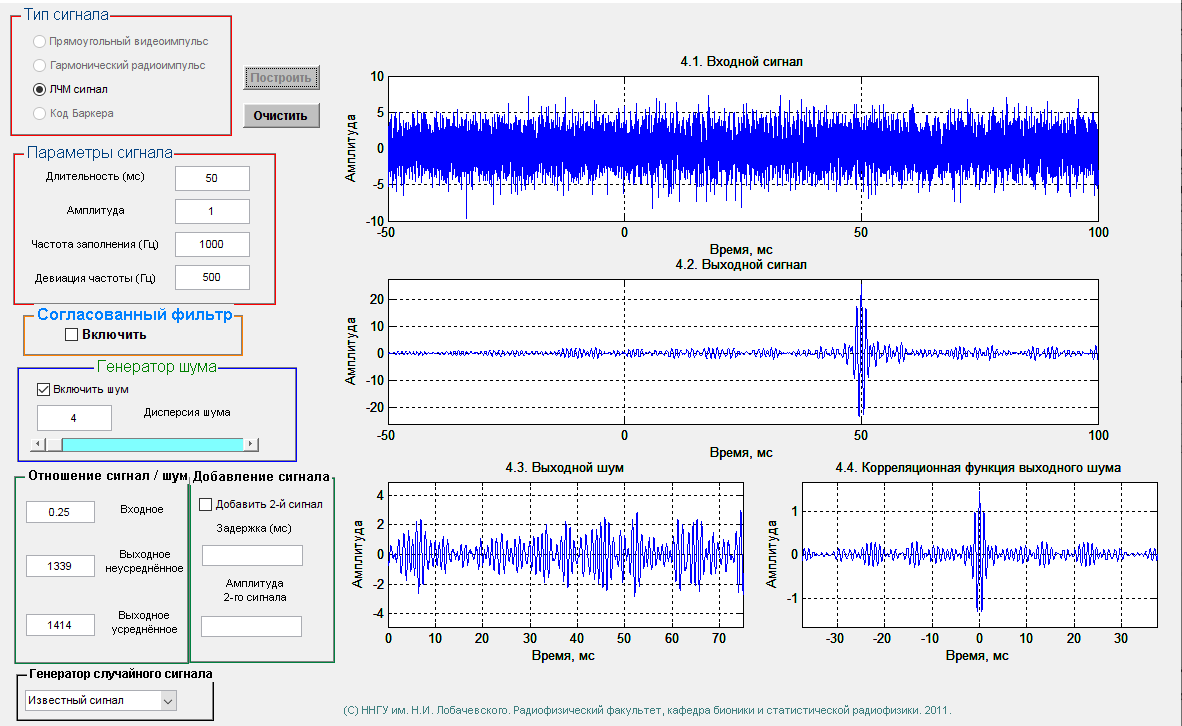
\includegraphics[width=0.6\linewidth]{imgs/t4s4_500}
    \includegraphics[width=0.6\linewidth]{example-image-a}
    \caption{Зависимость ОСШ от девиации частоты $\Delta f_{\text{дев}}$ ЛЧМ
    сигнала}
    \label{fig:4.1}
\end{figure}




